%!TEX root = ../paper.tex
The traditional approach taken in the study of chemical reaction, gene-regulatory, population, and ecosystem networks is to derive a system of differential equations to model a particular biological network, attempt to fit that model to data and adjust the modeling assumptions along with parameter values until a good fit is achieved \cite{Meyer2014}. All of these models utilize essentially equivalent mathematical structures, \ref{fig:biomodelexamples}, \cite{RossCr2003,Palsson2011a,Sauro2012}. Developing unified mathematical descriptions of all of these is one of the paramount goals of systems biology.
% \cite{RossCr2003,Alon2006,Palsson2006,HamidBolouri2008,Palsson2011a,Voit2012,Sauro2012}

Recent work has demonstrated that as a result of the existence of largely insensitive directions within the parameter space for such models, the approach outlined above often allows for a large variety of models to fit equivalent data \cite{Machta2013,Hines2014,Prabakaran2014,Tonsing2014}. In addition, there is often uncertainty about the very structure of such networks. In this context, it is crucial to gain insight into what dynamical phenomena are possible to observe within a given class of dynamical systems. This is necessary to understand in order to determine whether or not a particular dynamical phenomenon should be regarded as unique or generic in the development and investigation of models applied to particular systems \cite{Gunawardena2013,Gunawardena2014}. This can be achieved using a method common in statistical physics involving the consideration of an ensemble of systems that, in comparison to one another, appear to have components that are randomly interlinked.
% \cite{Brown2003,Gutenkunst2007,Daniels2008a,Machta2013,Hines2014,Prabakaran2014,Tonsing2014}

% Some conclusions derived from this approach may be sensitive to the probability distribution from which the strengths of interconnection are sampled, whereas others are independent of the specific form of this distribution. In the former case, discovering the constraints that contribute to determining the functional form of the distribution can be a matter for empirical investigation and results that are themselves functions of this distribution can be reinterpreted in light of ongoing updates from relevant empirical observations. On the other hand, results that are independent of the specific form of this distribution can be expected to hold in any case and a specific distribution may simply be chosen for the purposes of exemplifying the result.

Investigating generic properties of a large class of dynamical systems was the approach taken by May in models of ecosystem dynamics \cite{Gardner1970,May1972}. The class of dynamical systems studied by May is, however, not restricted to ecosystem dynamics and encompasses, among others, the dynamics of all of the networks represented in \ref{fig:biomodelexamples}. May conjectured on the basis of results from random matrix theory what eventually came to be referred to as the May-Wigner stability theorem \cite{Cohen1984,May1972a,Radius2014,Majumdar2014}, which implies a relationship between a topological property, system connectivity, and a dynamical property, stability.

% \begin{figure*}[!ht]
% \centering
% \noindent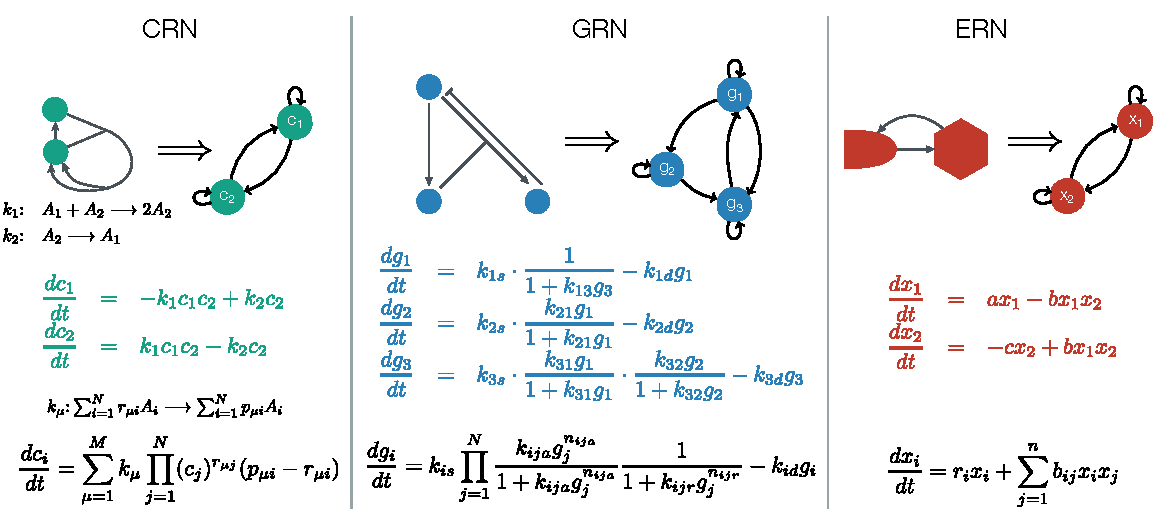
\includegraphics[width=0.8\textwidth]{fig/biomodelexamples.pdf}
% \caption{{\bf Dynamical models in systems biology.} The top row represents a chemical reaction network (CRN) \cite{Shinar2010}, a gene regulatory network (GRN) \cite{Karlebach2008}, and an ecological regulatory network (ERN) \cite{Rohr2014} in terms of the graphical methods specific to each field mapped into the interaction graph, which provides a unified representation for networks across these fields. The second row represents a particular example of a system of differential equations that are used to model a biological network within each of the domains of application considered here. The third row shows the general form of a system of differential equations that can be used to model any network architecture within each domain.}
% \label{fig:biomodelexamples}
% \end{figure*}

Here we determine the relationship between network hierarchy, a topological property, and the probability of \emph{robustness}, a dynamical property. Robustness is of interest in biological systems at all scales, and has been previously studied in the context of biochemical reaction networks \cite{Shinar2010}, gene-regulatory networks \cite{VanNimwegen1999,Siegal2002,Wagner2013}, and ecological networks \cite{Rohr2014}. For the purpose of this investigation, we quantify dynamical robustness as the probability of stability to potentially large perturbations of the parameters for systems which have already been determined to be stable in the sense of linear stability analysis \cite{Davis1962}. The maximally hierarchical network is considered to be the graph associated to the reflexive total ordering \cite{Cormen2009}. An example of this for three system components is shown in \reffigscc{} top. We use a measure of hierarchy based upon the edit distance from this maximally hierarchical network \cite{Axenovich2011}. We demonstrate that systems with the most hierarchical network topology according to this definition exhibit maximal robustness and explain why this results from an invariance of robustness to particular kinds of transformations of the network topology. Moreover these results hold for networks of arbitrary size and independent of the probability distribution from which the strengths of interaction are sampled.
% \cite{WADDINGTON1942a,VanNimwegen1999,Siegal2002,Ciliberti2007b,Ciliberti2007,Wagner2013}
